%-----------------------------------------------
% Dateiname: Doctrine.tex
% Autor    : Stefano Kowalke <blueduck@gmx.net>
% Lizenz   : BSD
%-----------------------------------------------
\section{Doctrine}
Das Doctrine Projekt besteht aus einer Reihe von PHP-Bibliotheken, die Schnittstellen rund um die Datenbankschicht bereitstellen. Die Konzepte sind beeinflusst von Javas \textit{Hibernate}\footnote{\url{http://hibernate.org/}} (vgl. \cite{web:t3nDoctrine2009}) und dem Entwurfsmuster \textit{Active Record}, welches von Martin Fowler \cite{book:fowlerPatterns2003} vorgestellt wird.

Das Projekt wurde 2006 von Konsta Vesterinen\footnote{\url{http://docs.doctrine-project.org/projects/doctrine1/en/latest/en/manual/acknowledgements.html}} initiiert und im Jahr 2008 als Version 1.0.0 veröffentlicht. Die Version 2.0 wurde im Jahr 2010 unter dem neuen Projektleiter Benjamin Eberlei fertiggestellt.

Die beiden bekanntesten Produkte des Projekts sind:
\begin{itemize}
	\item \gls{orm} - ermöglicht die objekrelationale Abbildung von Objekten auf Datenbanktabellen
	\item \gls{dbal} - stellt eine Datenbankabstraktionsschicht bereit
\end{itemize}

Wie aus Abbildung~\ref{fig:doctrineArchitecture} ersichtlich wird, ist Doctrine DBAL lediglich als eine dünne Schicht auf Basis der \gls{php}-Extension \gls{pdo} ausgeführt, die die grundlegenden Funktionen zur Abstraktion von Datenbanken implementiert. Die ORM Schicht baut auf Doctrine DBAL auf.

\begin{figure}[H]
    \centering
    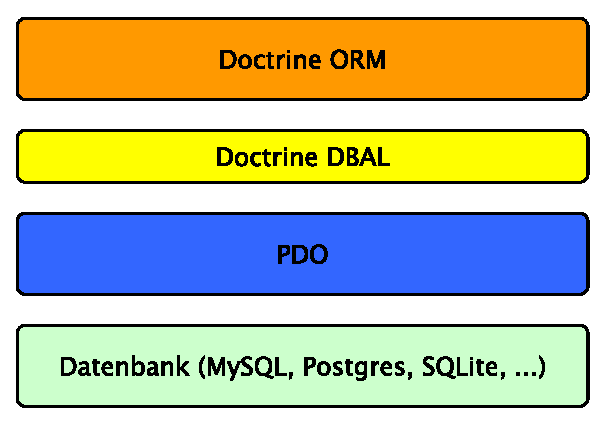
\includegraphics[scale=0.75]{diagrams/DoctrineArchitecture.eps}
    \caption{Schematischer Aufbau von Doctrine}
    \label{fig:doctrineArchitecture}
\end{figure}

\begin{shadequote}[l]{Jonathan Wage \cite{web:t3nDoctrine2009}}
	Ein ORM ist eine Abstraktionsschicht zwischen relationaler Datenbank und der eigentlichen Anwendung. Statt per SQL kann man durch das ORM objektorientiert auf die Daten zugreifen.
\end{shadequote}

Das folgende Anwendungsbeispiel zeigt eine typische Situation. Es wird zunächst ein neues Objekt eines Studenten erzeugt um im weiteren Verlauf mit verschiedenen Daten angreichert. Anschließend wird es als zu speicherndes Objekt bei der Datenbank registiert und schlußendlich gespeichert.

Im zweiten Codelisting wird die gleiche Aufgabe auf dem herkömmlichen Weg gelöst. Dabei wird die Anfrage an eine MySQL und PostgreSQL Datenbank gesendet. Die Variable \phpinline{$connection} enthält je eine initialisierte Verbindung zur entsprechenden Datenbank.

\begin{listing}
\begin{phpcode}
<?php

$student = new Student();
$student->setFirstName('Stefano');
$student->setLastName('Kowalke');
$student->setEnrolmentNumber('12345');
$entityManager->persist($student);
$entityManager->flush();
\end{phpcode}
\caption{Speichern eines Studenten in die Datenbank mit ORM}
\label{lst:orm}
\end{listing}

\begin{listing}
\begin{phpcode}
<?php

$sql =
    'INSERT INTO students ('first_name', 'last_name', 'enrolment_number')
    VALUES ('Stefano', 'Kowalke', '12345');

// MySQLi
$result = mysqli_query($connection, $sql);

// PostgreSQL
$result = pg_query($connection, $sql);

\end{phpcode}
\caption{Speichern eines Studenten in die Datenbank ohne ORM}
\label{lst:withoutOrm}
\end{listing}

Der Code in Listing~\ref{lst:orm} gibt keinen Rückschluss auf die darunterliegende Datenbank. Die Daten des Studenten könnten in eine CSV-Datei, einer MySQL oder Postgres Datenbank gespeichert worden sein. Hingegen wurden in Listing~\ref{lst:withoutOrm} zwei verschiedene Methoden genutzt, um die Daten in eine MySQL und Postgres Datenbank zu schreiben. Die Speicherung in eine Textdatei wurde dabei nicht berücksichtigt.

Doctrine ORM ist für die Umwandlung des \phpinline{$student}-Objekt in eine \gls{sql}-Abfrage zuständig. Die erzeugte Abfrage ist mit der aus Codebeispiel~\ref{lst:withoutOrm} vergleichbar. Die Konvertierung der Anfrage in die verschiedenen \gls{sql}-Dialekte\footnote{Als \gls{sql} Dialekt wird ein vom \gls{sql}-Standard abweichender Hersteller-spezifischer Sprachumfang bezeichnet. Ein Dialekt ist in der Regel kompatibel mit dem Standard und erweitert ihn um eigene Sprachkonstrukte.} erfolgt durch Doctrine DBAL.

Doctrine konvertiert das Schema anhand von sehr unterschiedlichen Merkmalen in das \gls{sql} der jeweilgen \gls{dbms}, die zum Verständnis einen etwas tieferen Einstieg in die Eigenheiten der \gls{dbms} erfordern. Da dies den Umfang der Arbeit überschreitet, wurden markante Beispiele gewählt, die den Sachverhalt verdeutlichen.

Datenbankschemas werden in Doctrine von der Klasse \phpinline{Schema} repräsentiert. Im Beispiel wird zunächst eine Instanz dieser Klasse erstellt und anschließend wird eine neue Tabelle und mehrere Tabellenspalten mit unterschiedlichen Datentypen angelegt. In Zeile 24 wird das Schema in eine \gls{sql}-Abfrage übersetzt. Davor existiert es lediglich als PHP-Objekt bis zum Ende der Laufzeit des Scripts.

Die Variable \phpinline{$myPlatform} enthält die Information über das aktuelle benutzte \gls{dbms}.

\begin{listing}[H]
\begin{phpcode}
<?php

$schema = new \Doctrine\DBAL\Schema\Schema();
$beUsers = $schema->createTable('be_users‘);
$beUsers->addColumn('uid', 'integer',
  array('unsigned' => TRUE, 'notnull' => TRUE, 'autoincrement' => TRUE)
);
$beUsers->addColumn('pid', 'integer',
  array('unsigned' => TRUE, 'default' => '0', 'notnull' => TRUE)
);
$beUsers->addColumn('username', 'string',
  array('length' => 50, 'default' => '', 'notnull' => TRUE)
);
$beUsers->addColumn('password', 'string',
  array('length' => 100, 'default' => '', 'notnull' => TRUE)
);
$beUsers->addColumn('admin', 'boolean',
  array('default' => '0', 'notnull' => TRUE)
);
$beUsers->setPrimaryKey(array('uid'));
$beUsers->addIndex(array('pid'), 'be_users_pid_idx');
$beUsers->addIndex(array('username'), 'be_users_username');

$queries = $schema->toSql($myPlatform);
\end{phpcode}
\caption{Erstellen eines Schemas mit Doctrine}
\label{lst:createSchema}
\end{listing}

Die beiden Listings \ref{lst:mysqlFromSchema} und \ref{lst:pgsqlFromSchema} zeigen den Inhalt von \phpinline{$queries} – einmal für MySQL und für PostgreSQL.

\begin{listing}[H]
\begin{mysqlcode}
// Der Inhalt von $queries für MySQL
CREATE TABLE `be_users` (
	`uid` int(10) unsigned NOT NULL AUTO_INCREMENT,
	`pid` int(10) unsigned NOT NULL DEFAULT '0',
	`username` varchar(50) COLLATE utf8_unicode_ci NOT NULL DEFAULT '',
	`password` varchar(100) COLLATE utf8_unicode_ci NOT NULL DEFAULT '',
	`admin` tinyint(1) NOT NULL DEFAULT '0',
	PRIMARY KEY (`uid`),
	KEY `be_users_pid_idx` (`pid`),
	KEY `be_users_username` (`username`)
) ENGINE=InnoDB AUTO_INCREMENT=2 DEFAULT CHARSET=utf8 COLLATE=utf8_unicode_ci;
\end{mysqlcode}
\caption{Das erstellte Schema als MySQL Anfrage}
\label{lst:mysqlFromSchema}
\end{listing}

\begin{listing}[H]
\begin{psqlcode}
// Der Inhalt von $queries für PostgreSQL
CREATE TABLE be_users (
	uid serial NOT NULL,
	pid integer NOT NULL DEFAULT 0,
	username character varying(50) NOT NULL DEFAULT ''::character varying,
	password character varying(100) NOT NULL DEFAULT ''::character varying,
	admin boolean NOT NULL DEFAULT false,
	CONSTRAINT be_users_pkey PRIMARY KEY (uid)
) WITH (
	OIDS=FALSE
);
\end{psqlcode}
\caption{Das erstellte Schema als PostgreSQL}
\label{lst:pgsqlFromSchema}
\end{listing}

Anhand der Beispiel kann folgendes abgeleitet werden:

\begin{itemize}
	\item die Deklaration von  mit \phpinline{integer ... auto_increment} wird nach \sqlinline{int(10) ... AUTO_INCREMENT} für MySQL und \sqlinline{serial} für PostgreSQL übersetzt
	\item die einfache Deklaration von \phpinline{INTEGER} wird nach \sqlinline{INT(10)} und \sqlinline{INTEGER} übersetzt
	\item \phpinline{string} wird nach \sqlinline{VARCHAR} bzw. \sqlinline{CHARACTER VARYING} übersetzt.
	\item \phpinline{boolean} wird nach \sqlinline{TINYINT(1)} für MySQL und \sqlinline{BOOLEAN} für Postgres übersetzt.
\end{itemize}

Dabei geben die Werte in Klammern die Länge des Datentyps an. Es ist zu beachten, dass die Länge für String-Typen eine andere Bedeutung hat, als für numerische Datentypen. Wird ein \sqlinline{VARCHAR} mit der Länge \textit{34} definiert, bedeutet dies, dass darin eine Zeichenkette mit maximal 34 Zeichen inklusive Leerzeichen gespeichert werden kann. Würde man auf den (vollkommen abwegigen) Gedanken kommen in dieser Spalte das Buch \textit{The Hitchhiker's Guide to the Galaxy} von Douglas Adams speichern zu wollen, würde der Inhalt wie folgt aussehen: ``Far out in the uncharted backwate'' \cite[S. 3]{book:adamsHitchhikers1995}

Bei numerischen Datentypen beschreibt der Wert allerdings die Anzeigenbreite - also die Anzahl der angezeigen Ziffern des gespeicherten Wertes. Sollte der in der Spalte gespeicherte Wert kleiner sein als die Länge der Anzeigenbreite, werden die restlichen Stellen nach links mit Leerzeichen aufgefüllt. Wurde die Option \sqlinline{ZEROFILL} gesetzt, werden die restlichen Stellen mit Nullen anstelle von Leerzeichen aufgefüllt. Der Wert beinflusst in keinster Weise den maximal speicherbaren Wert. In einer als \sqlinline{TINYINT} definierten Spalten können immer 256 Werte gespeichert werden. Unabhängig davon ob sie mit \sqlinline{TINYINT(1)} oder \sqlinline{TINYINT(4)} deklariert wurde.


Hier kann man die Unterschiede der verschiedenen Hersteller erkennen. Die Ursachen liegen darin begründet, dass die verschiedenen Hersteller eigene Features in ihre Datenbanken implementiert haben, oder sich die interne Verwaltung der Daten unterscheidet. Dies ist vergleichbar mit dem HTML-Standard und den Browser-spezifischen Tags. Als Stichwort sei hier SQLite genannt, die die Daten wahlweise in einer Datei oder im RAM speichert und sich somit grundsätzlich von Datenbanken wie MySQL, Postgres oder Oracle unterscheidet, die die Daten in mehren Dateien ablegen.

Datenbanken verwalten die Daten in Datentypen, wie es von typisierten Programmiersprachen wie C und C++ bekannt ist. Jedoch bieten nicht alle Hersteller die gleichen Typen an. So gibt es zum Beispiel keinen \textit{Boolean}-Typ in MySQL; jedoch in Postgres. Doctrines Repräsentation des Datenbankschemas ist generisch ausgestaltet, damit es den angebenen Datentyp in das Datenbank-spezifische Äqvivalent umsetzen kann.


Gibt es mehrere ähnliche Datentypen wie \sqlinline{TINYINT} und \sqlinline{INT} oder \sqlinline{VARCHAR} und \sqlinline{LONGTEXT}, trifft Doctrine die Entscheidung anhand der Länge des Datentyps. Wird keine Länge bei der Schemadeklaration angegeben, wird der Standardwert der jeweiligen Datenbank gewählt.

- Konfus: bit und boolean
- Tinyint = Boolena in MySQL
Als Grundlage der Länge eines Datentypes dient das Binärsystem, in dem es lediglich zwei Werte – 0 und 1 - gibt. Dies erlaubt die Abbildung der Zusände \textit{An} und \textit{Aus} oder \textit{Ja} und \textit{Nein}. Dies entspricht den Datentyp \textit{Boolean}. In der Regel müssen allerdings größere Werte gespeichert werden. Dazu werden acht Bits zu einem Byte zusammengefasst.



Zu beachten sind an diesem Beispiel die folgenden Besonderheiten:
\begin{itemize}
	\item Autoincrement - autoincrement / Serial
	\item Boolean - tinyint / Boolean
	\item string - varchar / charakter varying
	\item primary key - \sqlinline{PRIMARY KEY (`uid`)} / \sqlinline{CONSTRAINT be_users_pkey PRIMARY KEY (uid)}
	\item \phpinline{$beUsers->addIndex} - \sqlinline{KEY `be_users_pid_idx` (`pid`)} / Indices werden in Postgres gesondert verwaltet (Screenshot einfügen)
\end{itemize}
